\documentclass[../main.tex]{subfiles}
\begin{document}


This chapter %TODO ?
describes the design principles of our analysis tools (AT), 
which are responsible for extracting meaningful information from the aggregated logs from the filesystem, 
and further to structure this information in a way such that further operations are possible. 
If you just need instructions on how use those tools (e.g.\@ for extracting data as CSV), 
see \Cref{sec:analysisSetup,sec:analysisBasicUsage}.

\begin{figure}
\begin{center}
  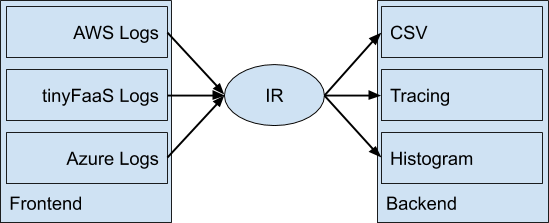
\includegraphics[width=\linewidth,keepaspectratio]{./IR-diagram.png}
\end{center}
\caption[Analysis Architecture Diagram]{%
Analysis Architecture Diagram. 
The frontend part is responsible for aggregating log output from all supported providers
and converting them all into a common format (IR). 
The backend processes can than perform various desired actions on this unified IR data.}%
\label{fig:analysisArchitectureDiagram}
\end{figure}

The analysis tools are split into two main parts. 
The first part (frontend) loads the log files and saves it in a common format, 
whereas the second part (backend) works on this common format and generates e.g.\@ graphs or CSVs
(see \Cref{fig:analysisArchitectureDiagram}).
Thus, the the frontend step only needs to be run once per test run.
Afterwards, we can then repeatedly execute backends against the extracted data.

\section{Frontend}%
\label{sec:analysisFrontend}

The frontend has to parse different log file formats from all supported providers 
which all provide the feature of extracting stdout to their individual logging service. 
The main framework is responsible for downloading those log files in any format and saving them into the local file system. 
The frontend then parses the events from all files into a list of structured events. 
It is important to export and work with the extracted data in various ways which require a different representation of the data. 
Thus, we have decided to introduce an intermediate representation from which each operation can extract their wanted representation. 
The main goal of the frontend is to run an ETL process on the logs and save all events and meaningful data in the IR output file.

%TODO check for changes

\end{document}
